\documentclass[10pt,hyperref={unicode}]{beamer}

%!TeX spellcheck = en-US,de-DE

%-------------------------------------------------------
% Beamer Theme location override
%-------------------------------------------------------

\makeatletter
  \def\beamer@calltheme#1#2#3{%
    \def\beamer@themelist{#2}
    \@for\beamer@themename:=\beamer@themelist\do%
    {\usepackage[{#1}]{\beamer@themelocation/#3\beamer@themename}}}

  \def\usefolder#1{
    \def\beamer@themelocation{#1}
  }
  \def\beamer@themelocation{}

%-------------------------------------------------------
% INCLUDE PACKAGES
%-------------------------------------------------------

\usepackage{minted} % Code listing new style
\usepackage{forest} % Tree graphs
\usepackage{fontspec} % UTf-8 input support lualatex
% \usepackage{multirow}
\usepackage{hyperref}
\usepackage{wasysym}
\usepackage[absolute,overlay]{textpos}
\usepackage{graphicx}
\usepackage{microtype} % nice text appearance
\usepackage{ragged2e}
\usepackage{pgfpages}
\usepackage[ngerman]{babel} % german text standards
\usepackage{docmute} % Import other .tex files ignoring document

%-------------------------------------------------------
% Config Theme
%-------------------------------------------------------
\usefolder{../Templates/featherZR}
\usetheme[
    progressstyle=movingCircCnt   % fixedCircCnt, movingCircCnt (moving is deault)
  ]{Feather}

\setsansfont{HelveticaNeue}
\setmonofont{Source Code Pro for Powerline}[Scale = MatchLowercase]

%-------------------------------------------------------
% DEFFINING AND REDEFINING COMMANDS
%-------------------------------------------------------

%Set Path to images
\graphicspath{{Images/}}

% colored hyperlinks
\newcommand{\chref}[2]{%
\href{#1}{{\usebeamercolor[bg]{Feather}#2} {\footnotesize\faExternalLink}}%
}

%Justification
\addtobeamertemplate{theorem begin}{}{\justifying}
\addtobeamertemplate{block begin}{}{\justifying}
\addtobeamertemplate{itemize begin}{}{\justifying}
\addtobeamertemplate{item begin}{}{\justifying}
\addtobeamertemplate{frame begin}{}{\justifying}
\addtobeamertemplate{quote begin}{}{\justifying}
\addtobeamertemplate{structure begin}{}{\justifying}

%etoolbox für nested list covering
\setbeamercovered{transparent}

%description inde
\setbeamersize{description width=0.57cm}

\makeatletter
\newcommand*\fix@beamer@close{%
  \ifnum\beamer@trivlistdepth>0
  \beamer@closeitem%
  \fi
}
\newcommand*\fix@beamer@open{%
  \ifnum\beamer@trivlistdepth>0
  \gdef\beamer@closeitem{}%
  \fi
}
\newcommand<>{\highlighton}[1]{%
  \alt#2{\structure{#1}}{{#1}}
}


\BeforeBeginEnvironment{enumerate}{\fix@beamer@close}
\AfterEndEnvironment{enumerate}{\fix@beamer@open}
\BeforeBeginEnvironment{itemize}{\fix@beamer@close}
\AfterEndEnvironment{itemize}{\fix@beamer@open}
\BeforeBeginEnvironment{description}{\fix@beamer@close}
\AfterEndEnvironment{description}{\fix@beamer@open}
\makeatother

% Codelistings
\definecolor{monokaibg}{HTML}{002833}
\definecolor{highlightbg}{HTML}{004550}

\setminted{
  autogobble=true,
  bgcolor=monokaibg,
  breaklines=true,
  fontsize=\footnotesize,
  highlightcolor=highlightbg,
  linenos=true,
  labelposition=bottomline,
  rulecolor=white,
  style=native,
}

\setmintedinline{
  bgcolor={},
  fontsize=\normalsize,
  style=manni
}

%-------------------------------------------------------
% INFORMATION IN THE TITLE PAGE
%-------------------------------------------------------

\title[Unit Tests ] % [] is optional - is placed on the bottom of the sidebar on every slide
{ % is placed on the title page
      \textbf{Mockery}
}

\subtitle[ -- Mocks für Tests in PHP]
{
%      \textbf{v. 1.0.0}
}

\author[Sebastian Knott]{Sebastian Knott}

\institute[]
{
      ZooRoyal IT\\

  %there must be an empty line above this line - otherwise some unwanted space is added between the university and the country (I do not know why;( )
}

\date{\today}

%-------------------------------------------------------
% THE TITLE OF THE PRESENTATION
%-------------------------------------------------------

\begin{document}

{\1
\begin{frame}[plain,noframenumbering] % the plain option removes the header from the title page, noframenumbering removes the numbering of this frame only
  \titlepage% call the title page information from above
\end{frame}}

\AtBeginSection[]
{
  \frame<handout:0>
  {
    \frametitle{Überblick}
    \tableofcontents[currentsection,hideothersubsections,sectionstyle=show/shaded,subsectionstyle=show/shaded]
  }
}

\AtBeginSubsection[]
{
  \frame<handout:0>
  {
    \frametitle{Überblick}
    \tableofcontents[currentsection,hideothersubsections,sectionstyle=show/shaded,subsectionstyle=show/shaded]
  }
}

\AtBeginSubsubsection[]
{
  \frame<handout:0>
  {
    \frametitle{Überblick}
    \tableofcontents[currentsection,hideothersubsections,sectionstyle=show/shaded,subsectionstyle=show/shaded,subsubsectionstyle=show/shaded]
  }
}

%-------------------------------------------------------
% THE BODY OF THE PRESENTATION
%-------------------------------------------------------

\begin{frame}
  \frametitle{Überblick}
  \tableofcontents[currentsection,sectionstyle=show,subsectionstyle=show,subsubsectionstyle=hide]
\end{frame}

\section{Was sind Doubles}


\begin{frame}
\frametitle{Double}
\framesubtitle{Begriffsklärung}
\begin{columns}[onlytextwidth]
  \begin{column}{0.5\textwidth}
    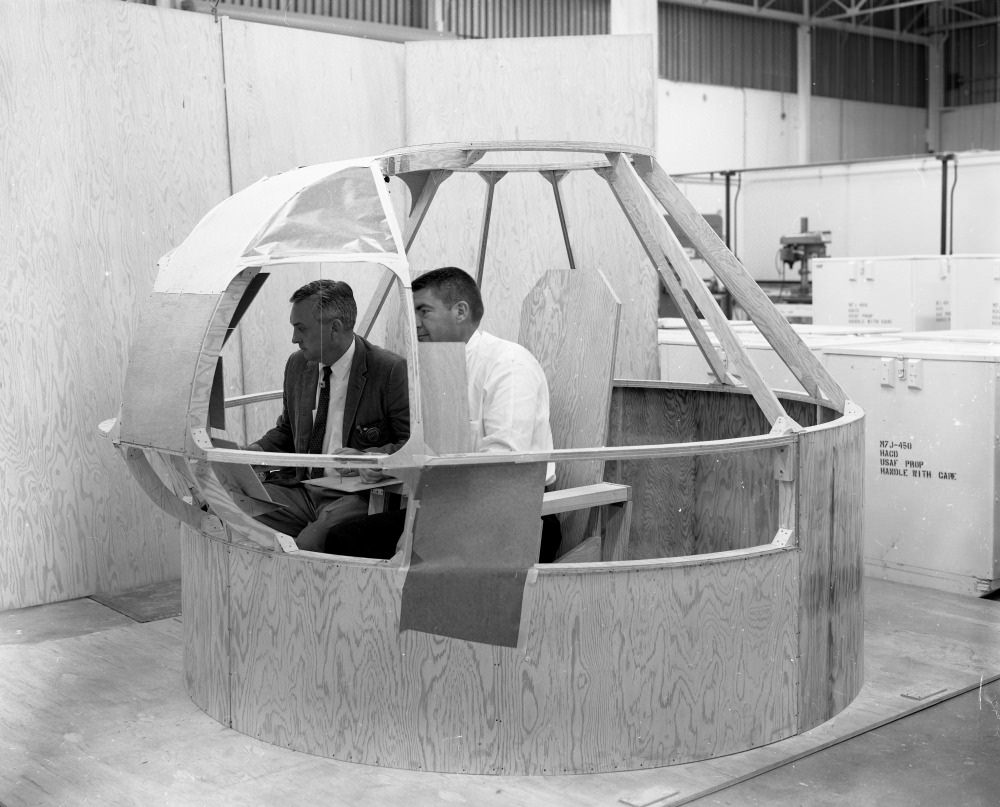
\includegraphics[width=0.9\textwidth]{double}
  \end{column}
  \begin{column}{0.5\textwidth}
    \begin{itemize}
      \item<+-> Doubles sind Objekte
      \item<+-> Ersetzen Klassen ohne Änderungen am Quellcode
      \item<+-> Weniger komplex als das Original
      \item<+-> Ermöglichen\dots
      \begin{itemize}
        \item<+-> Beobachten von Code
        \item<+-> Kontrolle über Programmfluss
      \end{itemize}
    \end{itemize}
  \end{column}
\end{columns}
\end{frame}


\section{Zweck von Doubles}


\begin{frame}[fragile]
\frametitle{Double}
\framesubtitle{Zweck von Doubles}

  Doubles spielen eine wichtige Rolle bei Unit-Tests.
  \begin{itemize}
    \item<+-> Abhängigkeiten des Testsubjekts werden durch Doubles ersetzt
    \item<+-> Subjekt wird vollständig isoliert (keine Nebeneffekte)
    \item<+-> Abhängigkeiten müssen nicht aufwendig erzeugt werden
    \item<+-> Interaktion des Subjekts mit den Doubles kann geprüft werden
  \end{itemize}

  \begin{minted}[firstline=2]{php}
    <?php
    protected function setUp()
    {
      $container = Mockery::mock(ContainerInterface::class);

      $subject = new MyClass($container);
    }
  \end{minted}
\end{frame}


\begin{frame}<handout:0>[label=fragen]
  \frametitle{Fragen}
  \framesubtitle{Fragen?}
  \begin{figure}
    \begin{center}
      
\includegraphics[height=4cm]{fragen}
    \end{center}
  \end{figure}
\end{frame}


\section{Mockery}


\begin{frame}[fragile]
\frametitle{Mockery}
\framesubtitle{WTF is Mockery?}

\begin{exampleblock}{}
  Mockery ist ein \highlighton{PHP-Mock-Framework}<+-> für PHPUnit, PHPSpec oder einem anderen Testframework. Sein Hauptziel ist es, ein Double-Framework mit einer \highlighton{prägnanten API}<+-> zu bieten, die in der Lage ist, alle möglichen Objektoperationen und -interaktionen unter Verwendung einer für \highlighton{Menschen lesbaren domänenspezifischen Sprache (DSL)}<+-> klar zu definieren. Entworfen als eine \highlighton{Alternative zur PHPUnit phpunit-mock-objects-Bibliothek}<+->, ist Mockery leicht mit PHPUnit zu integrieren und kann zusammen mit phpunit-mock-Objekten ohne, dass die Welt endet.
  \flushright{{\em -- \href{http://docs.mockery.io/en/latest/index.html}{Mockery.io}}}
  \end{exampleblock}

\end{frame}


\section{Arten von Doubles}
\subsection{Dummy}


\begin{frame}[fragile]
\frametitle{Dummy}

  Dummies sind leere Implementierungen einer Signatur einer Klasse.
  \begin{figure}
    \begin{center}
      Dummy Code
      \begin{minted}[firstline=2]{php}
        <?php
        class Container {
          public function __construct(DateTime $dateTime){}
          public function foo($targetFilePath){}
        }
      \end{minted}
    \end{center}
  \end{figure}


  \begin{figure}
    Test Code
    \begin{minted}[firstline=2]{php}
      <?php
      public function testArticle($targetFilePath){
        $container = new Container(new DateTime());
        $subject   = new MyClass($container)
        $subject->call();
      }
    \end{minted}
  \end{figure}

\end{frame}


\begin{frame}
\frametitle{Dummy}

  \begin{itemize}
    \item<+-> Aufwendig zu erzeugen
    \item<+-> Unflexibel
    \item<+-> Keine erweiterte Funktionalität
    \item<+-> Nur für einfachste Fälle praktikabel
  \end{itemize}
\end{frame}


\subsection{Stub}


\begin{frame}[fragile]
\frametitle{Stub}

  Stubs sind dynamisch erzeugte Objekte, vom Typ der Originalklasse.


    \begin{minted}[firstline=2]{php}
      <?php
      protected function setUp()
      {
        $container = Mockery::mock(Container::class);
        $subject   = new MyClass($container);
      }
    \end{minted}


  \begin{itemize}
    \item<+-> Sehr einfach zu erzeugen
    \item<+-> Keine erweiterte Funktionalität
    \item<+-> "'Quick and Dirty"'-Doubles.
  \end{itemize}

\end{frame}


\subsection{Mock}


\begin{frame}[fragile]
\frametitle{Mock}

  Mocks sind ebenfalls dynamisch erzeugte Objekte, vom Typ der Originalklasse. Mocks bieten erweiterte Funktionalität zur Simulation einer Klasse.

  \begin{minted}[firstline=2]{php}
    <?php
    protected function setUp()
    {
      $container = Mockery::mock(Container::class);
      $container->shouldReceive('foo')->once()
        ->with(stringValue)->andReturn(true);
      $subject   = new MyClass($container);
    }
  \end{minted}

  \begin{itemize}
    \item<+-> Einfach zu erzeugen
    \item<+-> Programmflusskontrolle
    \item<+-> Programmflussanalyse
    \item<+-> Konfiguration in komplexen Fällen umständlich
  \end{itemize}

\end{frame}


\subsection{Spy}


\begin{frame}[fragile]
\frametitle{Spy}

  Spies sind dynamisch erzeugte Objekte, vom Typ der Originalklasse. Sie agieren als Proxy zwischen Test und Originalklasse. Sie leiten Methodenaufrufe an das Original weiter und zeichnen die Interaktion zur späteren Analyse auf.

  \begin{minted}[firstline=2]{php}
    <?php
    protected function setUp()
    {
      $container= Mockery::spy(Container::class)->makePartial();
      $subject  = new MyClass($container);
      $subject->call();
      $container->shouldHaveReceived('foo');
    }
  \end{minted}

  \begin{itemize}
    \item<+-> Sehr einfach zu erzeugen
    \item<+-> Nachvollziehen des Programmflusses
    \item<+-> Bricht Isolation des Subjects
  \end{itemize}

\end{frame}


\section{Advanced Usage}
\subsection{Mock vs. Spy}


\begin{frame}[fragile]
\frametitle{Mock vs. Spy}
  \begin{minted}[firstline=2]{php}
    <?php
    $mock = Mockery::mock('MyClass');
    $spy  = Mockery::spy('MyClass')->makePartial();

    $mock->shouldReceive('foo')->andReturn(42);

    $mockResult = $mock->foo();
    $spyResult  = $spy->foo();

    $spy->shouldHaveReceived()->foo();

    var_dump($mockResult); // int(42)
    var_dump($spyResult); // original class result
  \end{minted}
\end{frame}


\subsection{Partial Mock}


\begin{frame}[fragile]
  \frametitle{Partial Mocks}
  \begin{figure}
    \begin{center}
      Test
      \begin{minted}[firstline=2]{php}
        <?php
        $mock = Mockery::mock('MyClass[foo,blub]',
          array($arg1, $arg2));

        $mock->shouldReceive('foo')->andReturn(42);

        $mockResult = $mock->bar();
      \end{minted}
    \end{center}
  \end{figure}

  \begin{figure}
    \begin{center}
      Subject
      \begin{minted}[firstline=2]{php}
        <?php
        class MyClass() {
          public function foo() {/* complex code */}
          public function bar() {
            foo();
          }
        }
      \end{minted}
    \end{center}
  \end{figure}
\end{frame}





\begin{frame}[plain]
 \begin{columns}[onlytextwidth]
   \begin{column}{0.5\textwidth}
     \begin{center}
        
\includegraphics[width=0.5\textwidth]{danke}
     \end{center}
   \end{column}
   \begin{column}{0.5\textwidth}
     Danke für eure Aufmerksamkeit!
   \end{column}
 \end{columns}
\end{frame}


\section{Code Dojo}
\subsection{Das Dojo}



{
\usebackgroundtemplate{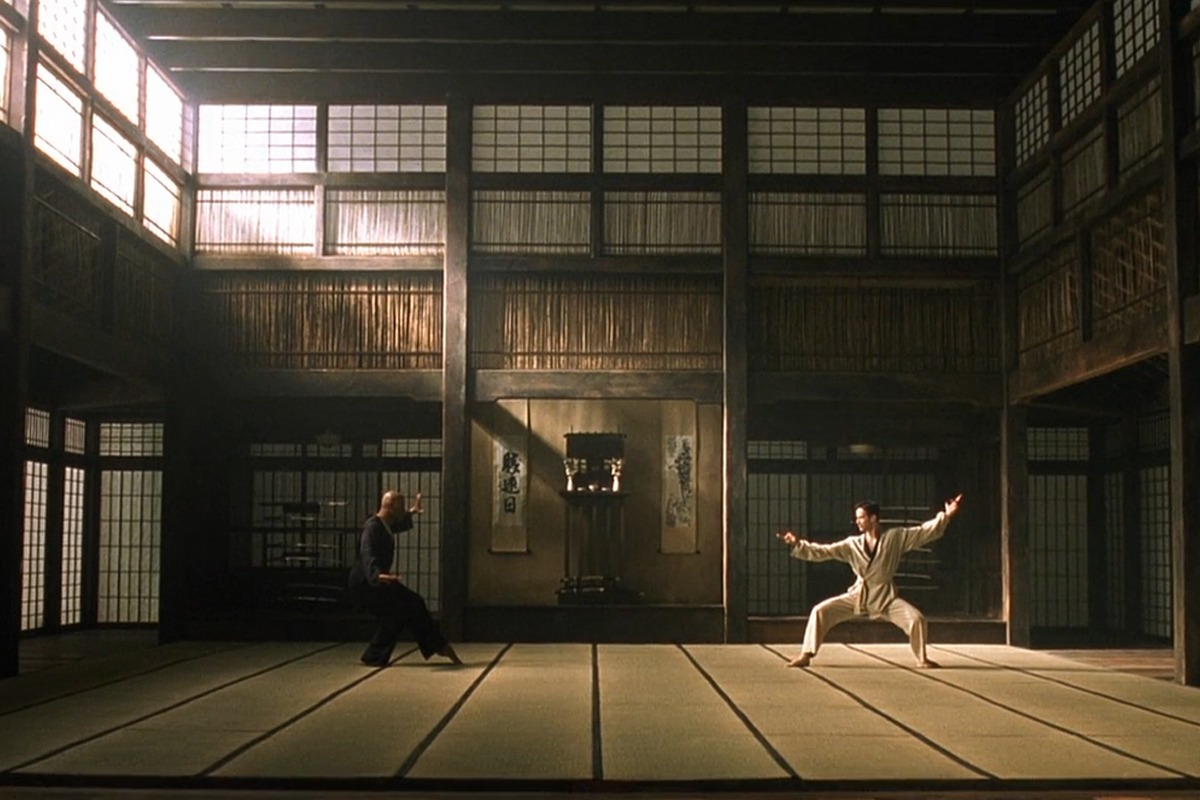
\includegraphics[height=\paperheight,width=\paperwidth]{dojo}}
\setbeamertemplate{blocks}[rounded][shadow=false]

  \begin{frame}[fragile]
    \frametitle{Code Dojo}
    \framesubtitle{Was ist ein Dojo?}
    \begin{exampleblock}{}
      Dojo (jap. Ort des Weges) bezeichnet einen Trainingsraum für verschiedene japanische Kampfkünste (Budo) [\dots]. Im übertragenen Sinne steht der Begriff auch für die Gemeinschaft der dort Übenden.
      \flushright{{\em Wikipedia}}
    \end{exampleblock}
  \end{frame}


  \begin{frame}[fragile]
    \frametitle{Code Dojo}
    \framesubtitle{Was ist ein Dojo?}

    \begin{exampleblock}{}
      Die Gemeinschaft führt gemeinsam Übungen -- so genannte Katas -- durch um ihr Wissen in der entsprechenden Disziplin zu vervollkommnen.
    \end{exampleblock}
  \end{frame}
}


\subsection{Code Kata}


\begin{frame}[fragile]
  \frametitle{Code Kata}
  \framesubtitle{Was ist ein Code Kata?}

  \begin{figure}
    \begin{center}
      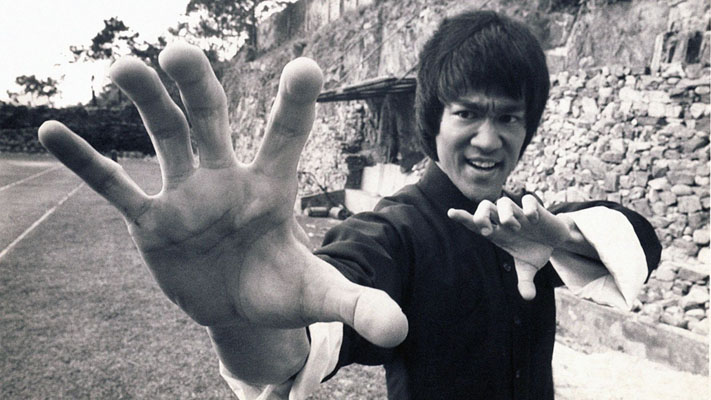
\includegraphics[width=0.7\textwidth]{bruce-lee}
    \end{center}
  \end{figure}

  \begin{itemize}
    \item<+-> Kleine, unabhängige, fokussierte, in sich geschlossene Übung
    \item<+-> Übt die Ausführung und Herangehensweise
    \item<+-> Bietet Raum für gemeinsames Lernen
    \item<+-> Lösung der Aufgabe erklärtes Nicht-Ziel
  \end{itemize}

\end{frame}


\subsection{Das Tennis Kata}

{
\usebackgroundtemplate{
\includegraphics[height=\paperheight,width=\paperwidth]{gears}}
\setbeamertemplate{blocks}[rounded][shadow=false]

\begin{frame}[fragile]
  \frametitle{Das Tennis Kata}
  \framesubtitle{Fokus}
  \begin{block}{Fokus}
    \begin{itemize}
      \item<+-> Pair Programming + TDD = TDD-Game
      \item<+-> Keine PHPMD Regel darf gebrochen werden
      \item<+-> Absichtsvolles Testen
      \begin{itemize}
        \item<+-> Test wird zuallererst dem Pair-Partner erklärt, dann programmiert
        \item<+-> Auswahl des Zwecks (use case, Erwartete Eingaben \dots)
        \item<+-> Auswahl der Kategorie (Black-, White-box)
        \item<+-> Gegebenenfalls Auswahl der Äquivalenzklasse.
      \end{itemize}
    \end{itemize}
  \end{block}

\end{frame}
}


{
\usebackgroundtemplate{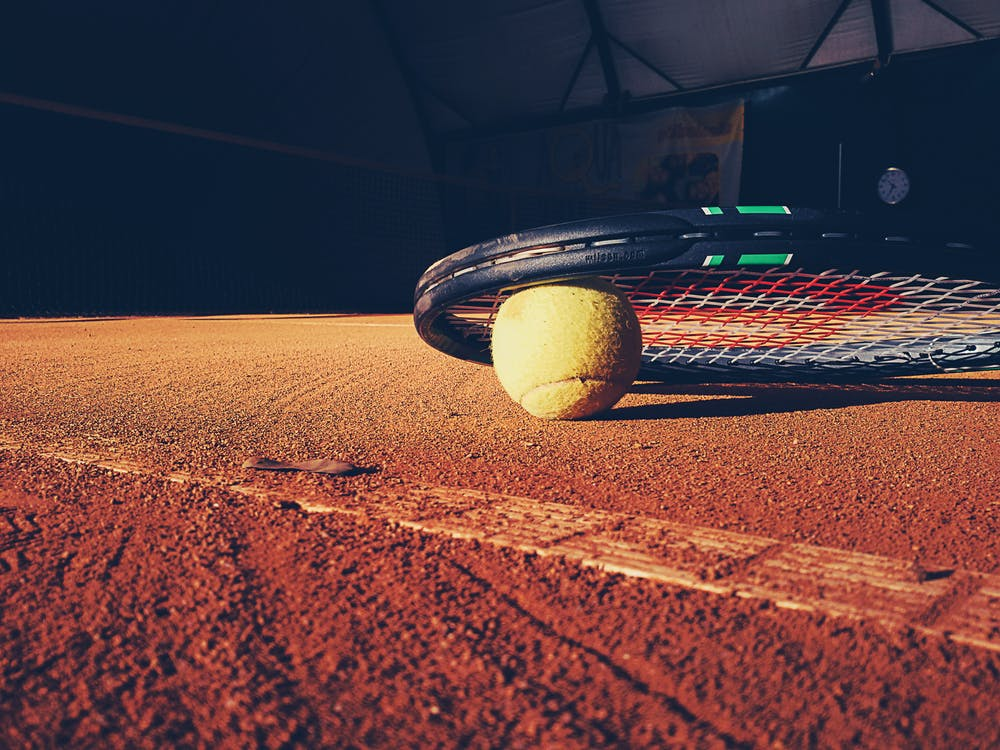
\includegraphics[width=\paperwidth]{tennis.jpg}}
\setbeamertemplate{blocks}[rounded][shadow=false]

\begin{frame}[fragile]

  \frametitle{Das Tennis Kata}
  \framesubtitle{Anforderung}

  \begin{block}{Anforderung}
    \begin{itemize}
      \item Eine Klasse muss die folgenden public Methoden haben
      \begin{itemize}
        \item \highlighton{addPointToPlayer(PlayerName:string):null} - Soll aufgerufen werden wenn ein Spieler einen Punkt erzielt. Wirft eine Exception, wenn das Spiel vorbei ist
        \item \highlighton{getCurrentScore():string} - Gibt eine Übersicht über alle gespielten Sätze, den aktuellen Punktestand und ob ein Spieler gewonnen hat aus.
        Es gelten die \href{https://de.wikipedia.org/wiki/Tennis#Gliederung_und_Zählweise}{Tennisregeln} mit 2 Gewinnsätzen.
      \end{itemize}
      \item Das Konzept des Tennisspieler muss in einer einzelnen Klasse \mintinline{php}|Player| implemtiert werden. Daten den Spieler betreffend müssen in \mintinline{php}|Player| gekapselt sein.
      \item Test-Subjects müssen vollständig isoliert sein
    \end{itemize}
  \end{block}

\end{frame}
}


%\begin{frame}
%  \frametitle{Danke}
%  \begin{columns}[onlytextwidth]
%    \begin{column}{0.5\textwidth}
%      \includegraphics[width=0.5\textwidth]{james}
%    \end{column}
%    \begin{column}{0.5\textwidth}
%      Danke für eure Aufmerksamkeit!
%    \end{column}
%  \end{columns}
%\end{frame}



%-------------------------------------------------------
% HELPER PAGES
%-------------------------------------------------------

\appendix

\begin{frame}<handout:0>[label=5minPause]
  \frametitle{Pause}
  \framesubtitle{5 Minuten Pause}
  \begin{figure}
    \begin{center}
      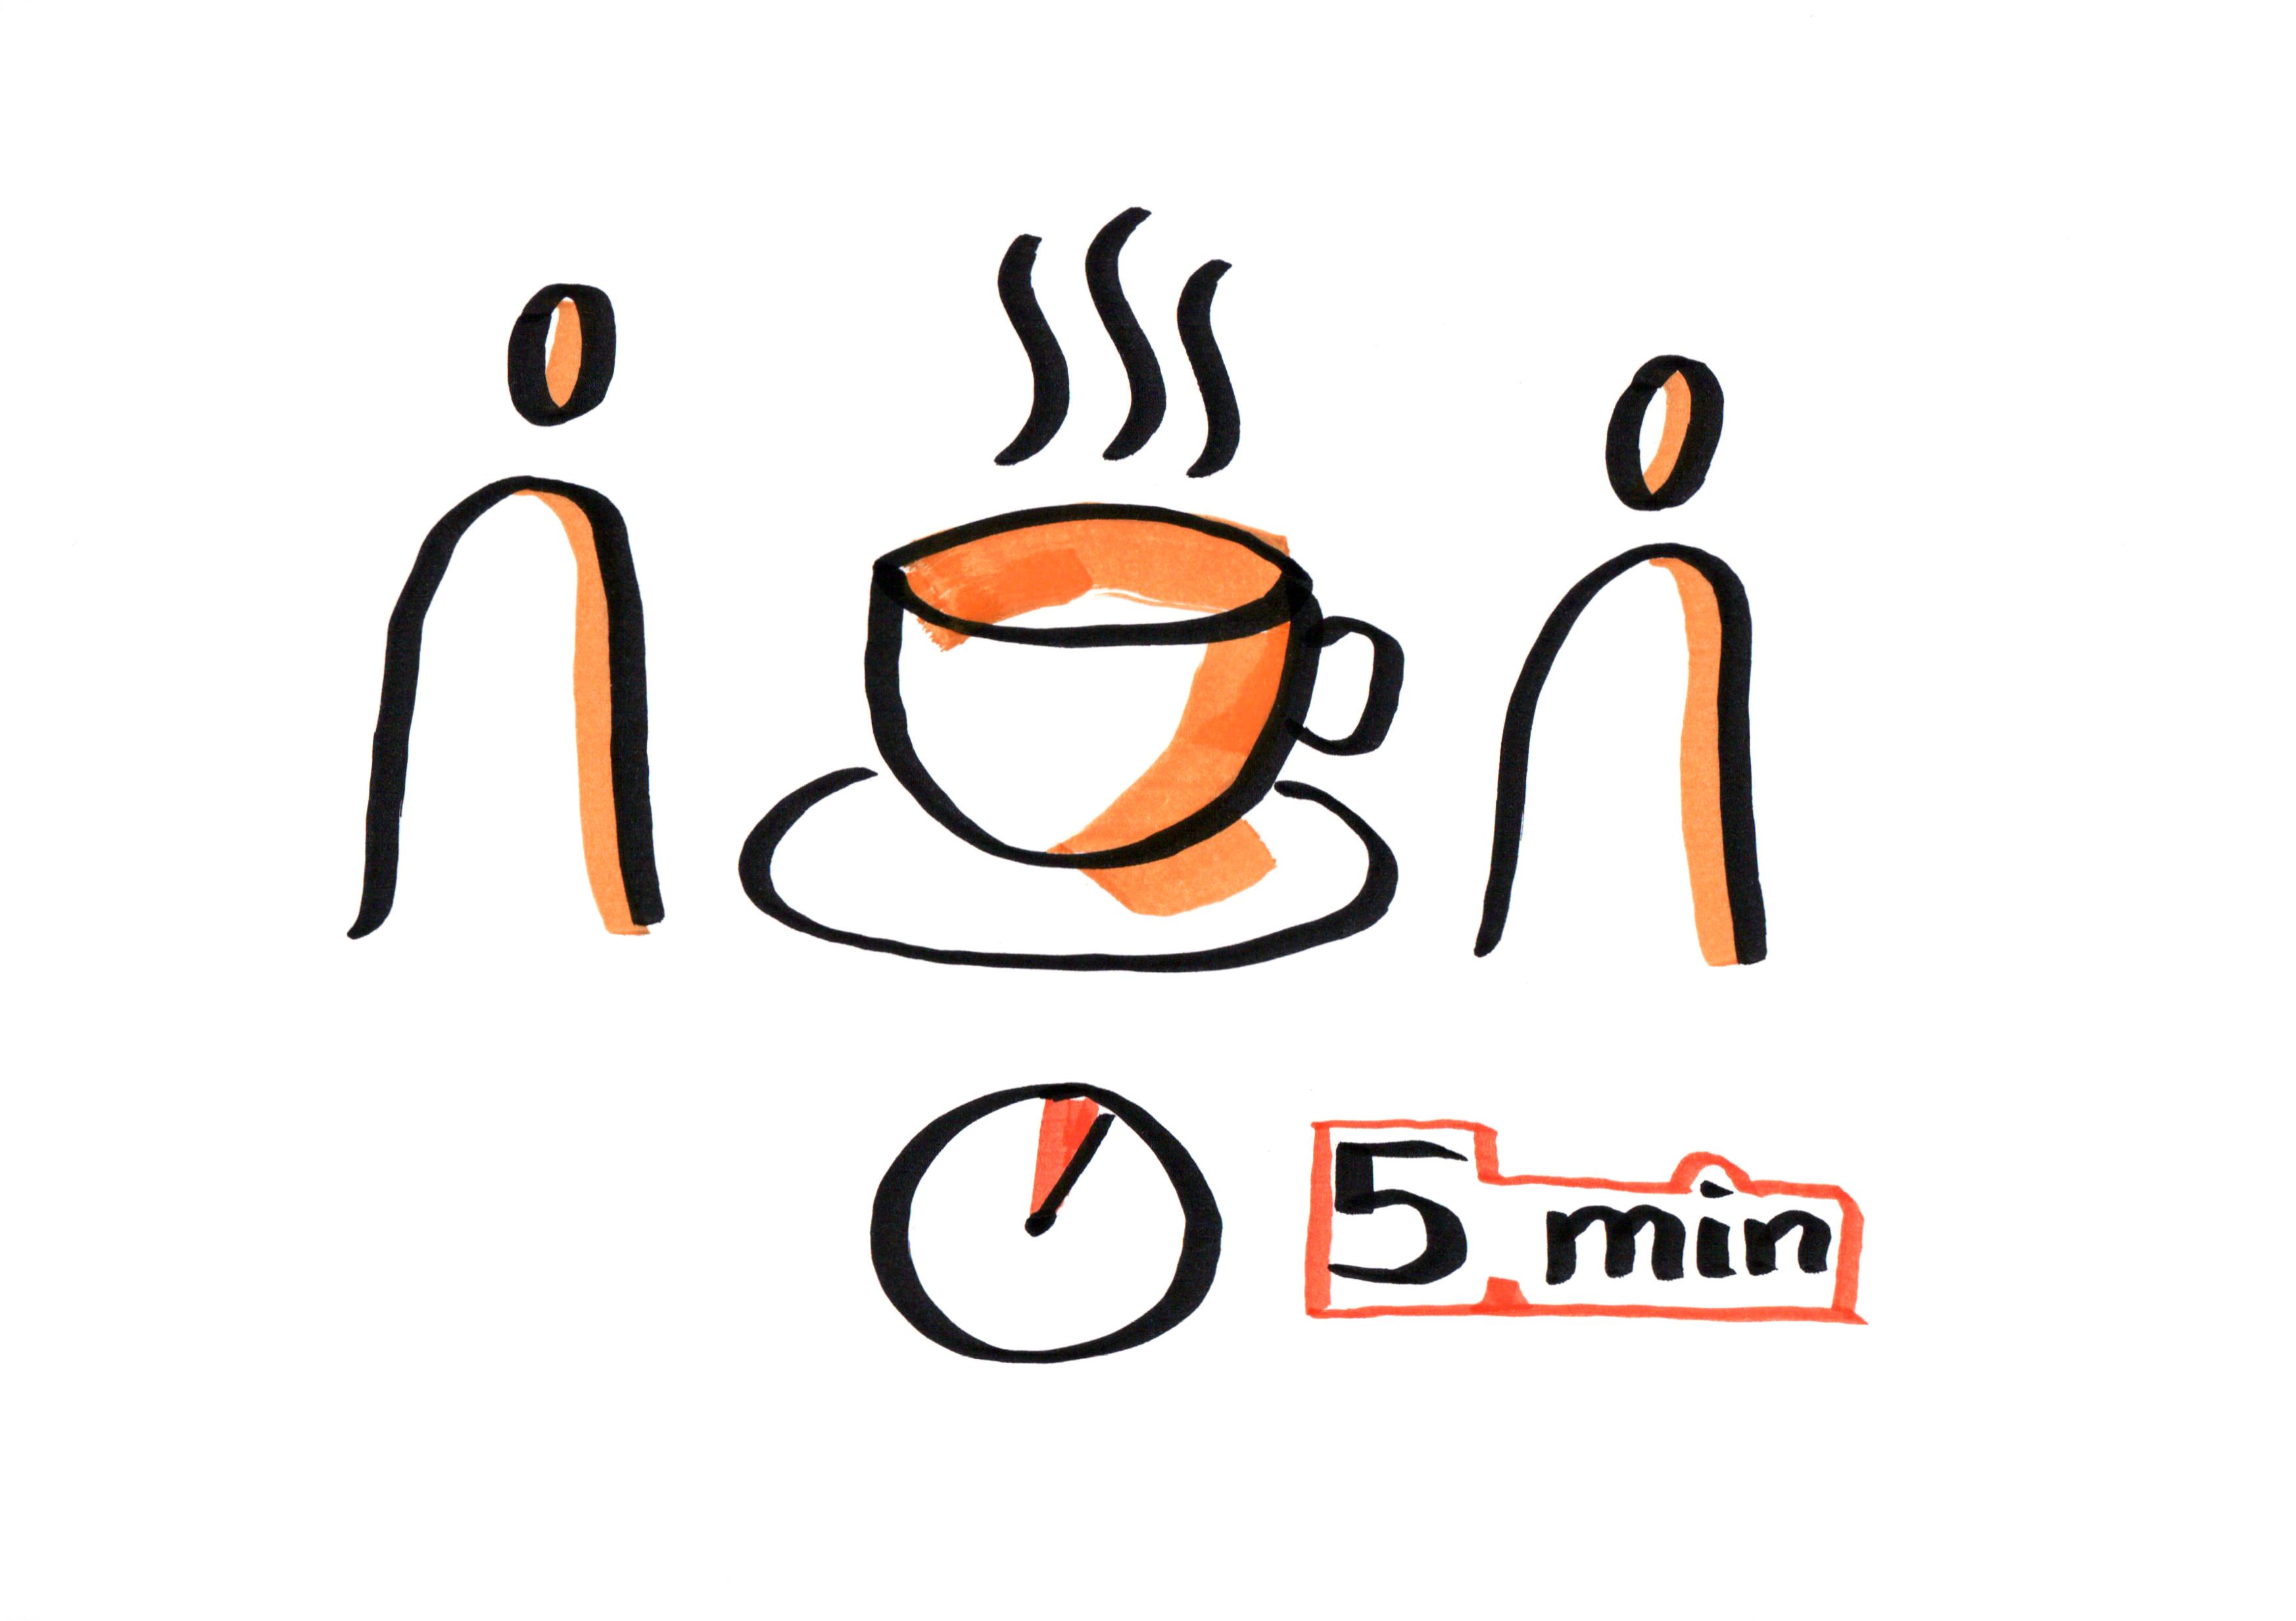
\includegraphics[height=4cm]{pause-5-min}
    \end{center}
  \end{figure}
\end{frame}



\begin{frame}<handout:0>[label=10minPause]
  \frametitle{Pause}
  \framesubtitle{10 Minuten Pause}
  \begin{figure}
    \begin{center}
      
\includegraphics[height=4cm]{pause-10-min}
    \end{center}
  \end{figure}
\end{frame}



\begin{frame}<handout:0>[label=pause]
  \frametitle{Pause}
  \framesubtitle{Pause}
  \begin{figure}
    \begin{center}
      
\includegraphics[height=4cm]{pause}
    \end{center}
  \end{figure}
\end{frame}



\begin{frame}<handout:0>[label=fragen]
  \frametitle{Fragen}
  \framesubtitle{Fragen?}
  \begin{figure}
    \begin{center}
      
\includegraphics[height=4cm]{fragen}
    \end{center}
  \end{figure}
\end{frame}



\end{document}
